\section{Regression Analysis}\label{Sec:Regression}

In order to analyze the effects of union coverage on wages and the wage distribution we will use three different econometric frameworks. Firstly, we will employ an OLS regression to investigate the effect on mean wages. However, the OLS regression framework of exploring the determinants of wages does not account for the possibility that covariates may have differential impacts across various parts of the wage distribution. Instead of focusing on the effect of union coverage on mean wages, the quantile regression approaches allow us to analyze the effects on different quantiles of the wage distribution. Hence, we can determine the contribution of union coverage to wage dispersion.

\subsection{OLS Regression}\label{SubSec:OLS}

\subsubsection{Theory}
We are interested in the effect of union coverage on wages. Let $ Y $ denote the outcome variable hourly wage and $ F_y(y) $ its distribution function, where $ F_y(y)=Pr(Y\leq y) $. $ X $ determines the union coverage status of one of the two union regimes (firm-level or sectoral-level) and is therefore a dummy variable, $ x= \{0,1\}$. $ Y_1 $ and $ Y_0 $ can be denoted as the possible outcomes under alternate values of $ X $. Hence, $Y=X\cdot Y_1 + (1-X)\cdot Y_0$, if union coverage is statistically independent of the possible outcomes. The unconditional distribution function for Y can be expressed as a weighted average of conditional distribution function of Y given X, weighted by the unconditional distribution of X \citep{Borah&Basu:2013}:

\begin{equation}\label{1}
  F_{y}(y)=Pr(X=1)F_{Y|X}(y|X=1) + Pr(X=0)F_{Y|X}(y|X=0)
\end{equation}

The ordinary least squares estimator gives us a consistent estimator of the target parameter $\beta_{OLS}$, that measures the effect of a marginal change in $X$ on the conditional expectation of $Y$, $\beta_{OLS}=\E[Y|X=1]-\E[Y|X=0]$. However, in most cases, useful interpretations can only be drawn from the effect of a change in the unconditional distribution of $X$ on the unconditional distribution of $Y$. One convenient feature of the OLS estimator is, that it is a consistent estimator for the effect on the unconditional distribution of $Y$ as well,\footnote{ This holds true as long as the estimated model is linear in all parameters.} because:
\begin{equation}\label{2}
  \E [Y]=p(X)\E[Y|X=1]+(1-p(X))\E[Y|X=0]
\end{equation}
\begin{equation*}
  \frac{d\E[Y]}{dp(X)}=\E[Y|X=1]- \E[Y|X=0]=\beta_{OLS}
\end{equation*}

Therefore, the coefficients obtained by OLS regression can be interpreted as the effect of a marginal change of $X$ on the unconditional mean of $Y$.

\subsubsection{Implementation}

\subsubsection{Testing - OLS Regression Results}
The regression of log hourly wages is done with respect to a set of covariates $ X \equiv [I, F, V] $, where $ I $ represents individual worker characteristics, such as education, years in the firm, gender and full-time working status. Firm characteristics are denoted by $ F $ and include, but are not limited to region and the share of female employees. $V$ refers to a vector of union coverage variables, containing (i) dummy variables for sectoral (SC) and firm-level (FC) coverage, (ii) variables for the share of employees within a firm, covered by either sectoral (shareSC) or firm-level (shareFC) collective contracts and (iii) interaction effects. The resulting regression can be expressed as:
\begin{equation}\label{OLS equation}
\begin{split}
   ln(w_{kn})= &  \beta_{0}+I_{kn}\beta_{X}+F_{n}\beta_{F} \\
   & +SC_{kn}\beta_{SC}+FC_{kn}\beta_{FC}+ shareSC_{n}\beta_{shareSC} +shareFC_{n}\beta_{shareFC}\\
   &  +SC_{kn} \cdot shareSC_{n}\beta_{shareSCxSC}+FC_{kn}\cdot shareFC_{n}\beta_{shareFCxFC} \\
\end{split}
\end{equation}
\begin{center}with $k=1,\dots , K$ individual employees and $n=1,\dots , N$ firms.\end{center}

The results of the OLS regression are presented in table \ref{OLS}. The regression results include a full set of firm-specific and individual covariates as well as different sets of union coverage variables. Specification (i) only includes the dummy variables for sectoral and firm-level collective coverage and suggests a union wage premium of $2.3\%$ for employees covered by a sectoral contract compared to employees without any collective bargaining contract. The union wage premium for employees under firm-level contracts is estimated to be even higher at $3.8\%$. Both effects are significant at the $1\%$-level.

Specification (ii) is restricted to the effect of the shares of covered employees within a firm on log wages. It turns out, that a $10\%$ increase in the share of covered employees within a firm yields on average a $0.53\%$ increase in wages for employees under sectoral collective coverage, and a $0.74\%$ increase for employees under a firm-level contract, respectively. Again, both effects are significant at the $1\%$ level.

In specification (iii), dummy variables for sectoral and firm-level coverage on an individual level as well as the firm-level coverage shares (shareSC and shareFC) are included. The individual coverage regime effects turn negative, whereas a higher share of covered employees in a firm is still associated with higher wages. In fact, the effects of higher coverage shares on wages increased to $0.94\%$ for a $10\%$ increase in the share of employees covered by a sectoral agreement ($1.92\%$ for a 10\% in crease in the share of employees covered by a firm-level agreement). Therefore, in a firm with close to $0\%$ coverage, union wage premiums turn negative. Conversely, in a firm with full coverage, the union wage premium is positive ($-0.041+100\% \cdot 0.094=0.053$ under sectoral contracts and $-0.113 +100\% \cdot 0.192=0.079$ under firm-level contracts).

Interaction effects between individual coverage and the share of covered employees in a firm are introduced in specification (iv). The individual coverage coefficients turn positive again and the effect of an increasing share of covered employees within a firm rises as well, compared to the other specifications. However, the interaction effects are estimated to be negative, suggesting that in firms with low coverage, individual coverage leads to higher wages than in firms with high coverage. The effect of individual coverage by a sectoral collective contract (firm-specific contract) in a firm with an average coverage ratio is $-2.5\%$\footnote{ $\beta_{SC}+\overline{shareSC}\cdot \beta_{shareSCxSC}=0.006- 0.357\cdot 0.087 =-0.025$} ($3.6\%$)\footnote{ $\beta_{FC}+\overline{shareFC}\cdot \beta_{shareFCxFC}=0.051-0.053 \cdot 0.276=0.036$}. Hence, an employee under a sectoral collective contract who works in a firm with an average coverage ratio earns $2.5\%$ less than an uncovered employee in the same firm. This may be due to a risk-premium paid to the uncovered workers since the negotiated wages for covered workers represent a wage floor. An alternative explanation might be the employee's preferences for performance pay. Conversely, an employee under a firm-specific contract in a firm with an average coverage ratio earns $3.6\%$ more than an uncovered employee in the same firm. This could be a result of firms hiring cheap labor (e.g. after leaving an employer's association), while the incumbent employees remain covered by the collective bargaining agreements. An increase in the share of covered employees results in a larger benefit for uncovered employees than for covered employees since the effect for covered employees is reduced by the coefficient of the interaction term. Thus, a $10\%$ increase in the coverage ratio of firms applying sectoral collective agreements leads to a $0.42\%$ increase in wages among covered employees and a $1.3\%$ increase in wages among uncovered employees. Similarly, for firms applying firm-specific agreements, a $10\%$ increase in the coverage ratio results in a $2.79\%$ increase in wages for uncovered employees, but has no effect for covered employees.

The difference between wages for male and female employees is significant and fairly constant across OLS regression specifications. On average, male employees earn almost $10\%$ more than female employees.

\newpage
\begin{landscape}
\begin{table}[]
\scriptsize
\centering
\caption{OLS Regression Results}
\label{OLS}
\begin{tabular}{l|cccccccc}
 & \multicolumn{2}{c}{i} & \multicolumn{2}{c}{ii} & \multicolumn{2}{c}{iii} & \multicolumn{2}{c}{iv} \\
\hline
variable & coef. & std. err. & coef. & std. err. & coef. & std. err. & coef. & std. err. \\
\hline
Sector Contract (SC)    & $0.023^{**}$ & $(0.001)$ &  &  & $-0.041^{**}$ & $(0.003)$ & $0.006^{*}$ & $(0.003)$\\
Firm Contract (FC)      & $0.038^{**}$ & $(0.002)$ &  &  & $-0.113^{**}$ & $(0.005)$ & $0.051^{**}$ & $(0.007)$\\
shareSC                 &  &  & $0.053^{**}$ & $(0.001)$ & $0.094^{**}$ & $(0.003)$ & $0.129^{**}$ & $(0.005)$\\
shareFC                 &  &  & $0.074^{**}$ & $(0.002)$ & $0.192^{**}$ & $(0.006)$ & $0.279^{**}$ & $(0.008)$\\
shareSCxSC              &  &  &  &  &  &  & $-0.087^{**}$ & $(0.006)$\\
shareFCxFC              &  &  &  &  &  &  & $-0.276^{**}$ & $(0.012)$\\
gender (0=male)         & $-0.096^{**}$ & $(0.001)$ & $-0.097^{**}$ & $(0.001)$ & $-0.095^{**}$ & $(0.001)$ & $-0.095^{**}$ & $(0.001)$\\
\hline
$R^{2}$                 & \multicolumn{2}{c}{$0.6258$} & \multicolumn{2}{c}{$0.6271$} & \multicolumn{2}{c}{$0.6278$} & \multicolumn{2}{c}{$0.6285$}  \\
$N$                     & \multicolumn{2}{c}{$552750$} & \multicolumn{2}{c}{$552750$} & \multicolumn{2}{c}{$552750$} & \multicolumn{2}{c}{$552750$}  \\
\hline
\end{tabular}\\
\bigskip
OLS regression includes a full set of firm-specific and individual covariates.\\
$^{*}$/$^{**}$: significance at the 5\%/1\% -level
\end{table}

\begin{table}[]
\scriptsize
\centering
\caption{Conditional Quantile Regression Results}
\label{CQR}
\begin{tabular}{l|cccccccccc}
 percentile & \multicolumn{2}{c}{(10)} & \multicolumn{2}{c}{(25)} & \multicolumn{2}{c}{(50)} & \multicolumn{2}{c}{(75)} & \multicolumn{2}{c}{(90)}\\
\hline
                & coef.             & std. err. & coef.     & std. err.         & coef.             & std. err. & coef.         & std. err. & coef.         & std. err. \\
\hline
Sector Contract (SC)    & $0.108^{**}$      & $(0.004)$ & $0.066^{**}$   & $(0.003)$    & $0.015^{**}$      & $(0.003)$ & $-0.031^{**}$ & $(0.004)$ & $-0.069^{**}$ & $(0.004)$\\
Firm Contract (FC)      & $0.152^{**}$      & $(0.010)$ & $0.129^{**}$   & $(0.009)$    & $0.066^{**}$      & $(0.007)$ & $0.030^{**}$  & $(0.008)$ & $0.015$       & $(0.013)$\\
shareSC                 & $0.174^{**}$      & $(0.007)$ & $0.218^{**}$   & $(0.004)$    & $0.225^{**}$      & $(0.004)$ & $0.224^{**}$  & $(0.004)$ & $0.211^{**}$  & $(0.007)$\\
shareFC                 & $0.244^{**}$      & $(0.011)$ & $0.291^{**}$   & $(0.009)$    & $0.318^{**}$      & $(0.011)$ & $0.349^{**}$  & $(0.011)$ & $0.350^{**}$  & $(0.021)$\\
shareSCxSC              & $-0.123^{**}$     & $(0.008)$ & $-0.180^{**}$  & $(0.005)$    & $-0.194^{**}$     & $(0.006)$ & $-0.190^{**}$ & $(0.006)$ & $-0.175^{**}$ & $(0.008)$\\
shareFCxFC              & $-0.272^{**}$     & $(0.017)$ & $-0.348^{**}$  & $(0.014)$    & $-0.346^{**}$     & $(0.012)$ & $-0.358^{**}$ & $(0.014)$ & $-0.349^{**}$ & $(0.025)$\\
gender (0=male)          & $-0.055^{**}$    & $(0.001)$ & $-0.056^{**}$  & $(0.001)$    & $-0.068^{**}$     & $(0.001)$ & $-0.087^{**}$ & $(0.001)$ & $-0.111^{**}$ & $(0.002)$\\
\hline
$N$                     & \multicolumn{2}{c}{552750} & \multicolumn{2}{c}{552750} & \multicolumn{2}{c}{552750} & \multicolumn{2}{c}{552750} & \multicolumn{2}{c}{552750} \\
\hline
\end{tabular}\\
\bigskip
Conditional quantile regression includes a full set of firm-specific and individual-worker covariates.\\
$^{*}$/$^{**}$: significance at the 5\%/1\% -level
\end{table}
\end{landscape}


\subsection{Conditional Quantile Regression}\label{SubSec:CQR}

\subsubsection{Theory}
The conditional quantile regression approach has been widely used in empirical analysis in order to assess the impact of covariates on different points of the distribution of the outcome variable $Y$. In line with the empirical investigation at hand, conditional quantile regression can help to study the effect of different determinants on wages for people along the wage distribution, since the effect of a covariate on lower quantiles may differ from the effect on higher quantiles. OLS regression does not account for those differences.

Analogously to equation \ref{1} for the OLS regression, we can develop the same approach for the $\tau$th-quantile, $q_{Y}(\tau)$, of the unconditional distribution of $Y$, where $\tau=F_{Y}(q_{Y}(\tau))$:

\begin{equation}\label{3}
  F_{Y}(q_{Y}(\tau))=Pr(X=1)F_{Y|X=1}(q_{Y}(\tau))+Pr(X=0)F_{Y|X=0}(q_{Y}(\tau)).
\end{equation}

Using implicit differentiation of equation \ref{3}, we can develop an expression for the unconditional quantile $\frac{dq_{\tau}}{dp(X)}$:
\begin{equation*}
  \frac{dF_{Y}(q_{Y}(\tau))}{dp(X)}=\frac{\partial F_{Y}(q_{\tau})}{\partial q_{Y}(\tau)}\cdot \frac{dq_{Y}(\tau)}{dp(X)}
\end{equation*}
\begin{equation*}
  F_{Y|X=1}(q_{Y}(\tau))-F_{Y|X=0}(q_{Y}(\tau))=f_{Y}(q_{\tau})\cdot \frac{dq_{Y}(\tau)}{dp(X)}
\end{equation*}
\begin{equation}\label{4}
  \frac{dq_{Y}(\tau)}{dp(X)}=\frac{F_{Y|X=1}(q_{Y}(\tau))-F_{Y|X=0}(q_{Y}(\tau))}{f_{Y}(q_{\tau})}
\end{equation}

When no other covariates are included in the regression model, the conditional effect equals the unconditional effect of a dummy variable for any quantiles of $Y$. Even if other covariates are included in the regression model, but the conditional effect does not depend on the distribution of the other covariates, conditional and unconditional treatment effects coincide for any quantile. Conversely, if the conditional treatment effect of $X$ varies over values of other covariates, conditional and unconditional effects will be likely to differ \citep{Borah&Basu:2013}.

The Conditional Quantile Regression approach was firstly introduced by \cite{Koenker&Bassett:1978}. Let $Q_{\tau}(Y|Z) = Z^{'}\beta_{\tau}^{CQR}$ be the quantile, conditioned on the vector of covariates $Z$, such that $Q_{\tau}(Y|Z)=F^{-1}(\tau)=\inf_{q}\{q:F_{Y|Z}(q|Z)\geq\tau\}$ \citep{Borah&Basu:2013}.\footnote{ $\inf\{\}$ refers to the infimum operator defining the greatest value of $q$ that still represents a lower bound in the set $F_{Y|Z}(q|Z)\geq\tau$}

In contrast to the OLS regression, in which the sum of squared residuals is minimized in order to obtain the $\beta_{OLS}$-vector, the vector of $\beta_{\tau}$ results from minimizing an asymmetric absolute loss function (i.e. the sum of weighted absolute residuals) \citep{Koenker&Bassett:1978}:

\begin{equation}\label{5}
  \min_{\beta_{\tau}\in R^{p}}\sum_{i=1}^n \rho_{\tau}(y_{i}-z_{i}^{'}\beta_{\tau})
\end{equation}
\begin{center}
with $\rho_{\tau}(u)=u\cdot (\tau-I(u<0))$, $\forall \tau \in (0,1)$
\end{center}
\begin{equation}\label{6}
  \Longrightarrow \min_{\beta_{\tau}\in R^{p}}\sum_{y_{i}\geq Z_{i}^{'}\beta}\tau \cdot \left| (y_{i}-Z_{i}^{'}\beta) \right| + \sum_{y_{i} < Z_{i}^{'}\beta}(1-\tau) \cdot \left| (y_{i}-Z_{i}^{'}\beta) \right|
\end{equation}

Following from equation \ref{6}, the so-called ''check function'' or absolute value function \citep{Koenker&Hallock:2001}, $\rho_{\tau}$ yields the $\tau$-th sample quantile as its solution as it weights the residuals $\left| (y_{i}-Z_{i}^{'}\beta) \right|$ with $\tau$ if they are positive, and with $(1-\tau)$ if they are negative. For $\tau=0.5$, positive and negative residuals are weighted equally and the sum of absolute deviations is minimized. For any $\tau > 0.5$ large positive errors are more heavily penalized than negative errors. The estimated coefficients $\hat{\beta_{\tau}}$ can be interpreted as marginal or partial effects on the conditional quantile $\tau$ for continuous and dummy variables, respectively.\\
The coefficient for a dummy covariate estimated in a conditional quantile regression is given by
\begin{equation}\label{7}
  \beta_{\tau}^{CQR}=F_{Y|X=1 , W=\bar{\omega}}^{-1}(\tau) - F_{Y|X=0 , W=\bar{\omega}}^{-1}(\tau)
\end{equation}
and conditioned on the vector of sample means $\bar{\omega}$ of all other covariates $W$. In general, the conditional effect of $X$ on $Y$ does not equal the unconditional effect of $X$ on $Y$ if the conditional effect of $X$ depends on the levels of other covariates $W$:
\begin{equation*}
  F_{Y|X=1 , W=\bar{\omega}}^{-1}(\tau)=q_{Y|X=1 , W=\bar{\omega}}(\tau) \neq q_{Y}(\tau)
\end{equation*}
Therefore, the coefficients obtained by a conditional quantile regression are to be interpreted as the effects on the conditional quantile, conditioned on the distribution of all other covariates.

\subsubsection{Implementation}

\subsubsection{Testing - Conditional Quantile Regression Results}
As pointed out in \cite{Fitzenberger&Kohn&Lembcke:13}, there is a variety of reasons why the coverage regime affects parts of the entire wage distribution differently. For example, union policy is usually oriented towards benefiting low-wage employees, bringing us to expect larger effects of union coverage on lower quantiles of the wage distribution. Moreover, we can assess the ambiguous effect uncovered workers face in partly covered firms across quantiles. On the one hand, uncovered workers may receive lower wages if the firm takes advantage of the possibility of hiring cheap labor. On the other hand, uncovered employees could possibly earn higher wages if firms decide to pay highly productive workers more than what has been settled in the collective contract. As stated above, the wage premium of uncovered employees could also represent a risk-premium as they cannot rely on contract wages as a fall back position.

In order to study the effect of different determinants on wages for people along the wage distribution I employ quantile regressions. The results of the conditional quantile regression are summarized in table \ref{CQR}. The manually calculated conditional average partial effects\footnote{ Calculated at the mean coverage rates of firm-specific/sectoral contracts: e.g. for individual coverage at the sectoral level (10th percentile): $\beta_{SC}^{(10)}+\overline{shareSC}\cdot \beta_{shareSCxSC}^{(10)}=0.108-0.357 \cdot 0.123=0.064$} are displayed in table \ref{APEs:CQR}. Please note that the conditional average partial effect refers to an average partial effect, conditioned on the distribution of all other covariates. In the following, if not stated otherwise, all regression coefficients obtained by conditional quantile regression refer to the effects conditioned on the distribution of all other covariates.

The median coefficients regarding employees, covered by a firm-level contract, are slightly higher than those obtained by the OLS regression, i.e. the conditional average partial effect of individual coverage by a firm-level contract is $4.8\%$ at the median (compared to $3.6\%$ from OLS regression) and an increase of $10\%$ in the share of covered employees within a firm with an average coverage ratio is estimated to increase wages by $3\%$ (compared to $2.6\%$ from OLS regression) at the median. However, regression coefficients for sectoral-level contracts differ in different directions from the OLS estimates. Increasing the share of covered employees by $10\%$ within a firm with an average coverage ratio results in a $1.6\%$ increase in wages at the median (a $1\%$ increase at the mean). Conditional quantile regression at the median yields a $-5.4\%$ conditional average partial effect for individual coverage by a sectoral collective agreement, whereas the OLS regression estimates suggest only a $-2.5\%$ union wage premium.\footnote{ A negative union wage premium means that uncovered workers earn more than covered workers.} Considering the overall declining tendency of the coefficient for individual coverage by a sectoral agreement across quantiles, the regression results suggest that the median of log wages is higher than the mean of log wages, which might be contra-intuitive since the wage distribution is usually skewed right (positively skewed). In fact, our sample confirms that mean log wages are lower than median log wages for sectoral coverage ($\overline{ln(w)}=2.859<2.877=ln(w)_{0.5}$), mean wages, however, are above median wages ($\overline{w}=19.04>17.76=w_{0.5}$).

\begin{table}[]
\scriptsize
\centering
\caption{Average Partial Effects obtained by Conditional Quantile Regression}
\label{APEs:CQR}
\begin{tabular}{l|ccccc}

                    & $(10)$ & $(25)$ & $(50)$ & $(75)$ & $(90)$ \\
  \hline
  Sector Contracts  & $0.064$ & $0.002$ & $-0.054$ & $-0.099$ & $-0.131$ \\
  Firm Contracts    & $0.138$ & $0.109$ & $0.048$ & $0.011$ & $0.003$ \\
  shareSC           & $0.130$ & $0.154$ & $0.156$ & $0.156$ & $0.149$ \\
  shareFC           & $0.230$ & $0.273$ & $0.300$ & $0.330$ & $0.332$ \\
  \hline
\end{tabular}
\end{table}

The effect of an increasing coverage share at the firm level rises along the conditional wage distribution for firms, that apply firm-specific collective contracts. Therefore, wages on higher quantiles are estimated to respond stronger to an increase in the coverage share within a firm, compared to lower quantiles. As a result, an increasing share of covered employees tends to contribute to wage dispersion in firms with firm-specific contracts. The effect of applying a sectoral collective contract within a firm remains fairly the same across the entire wage distribution. Thus, increasing the share of covered employees within a firm that applies sectoral collective contracts increases wages for low-wage earners similarly to those of high-wage earners, compared to a situation of no coverage.

The positive effect of sectoral or firm-level coverage, compared to no coverage, is declining along the wage distribution. The coefficient of individual coverage by firm-level contracts remains positive along the whole conditional wage distribution, whereas individual coverage by a sectoral collective agreement has a positive effect on lower conditional quantiles and a negative effect on higher conditional quantiles. Hence, individual coverage by any of the two bargaining regimes tends to reduce wage dispersion.

The inclusion of interaction effects in the regression model also allows us to analyze the different effects for individual coverage in high-coverage firms, compared to low-coverage firms. For low-coverage firms (coverage rate close to zero), the regression coefficients for (SC) and (FC) from table \ref{CQR} represent the effect of individual coverage on the conditional wage distribution. The effect of individual coverage for employees in high-coverage firms (coverage rate close to one) is reduced by the interaction coefficient. Table \ref{PEs:CQR:LH} summarizes the effects of individual coverage by sectoral and firm-level contracts on the conditional wage distribution in high-coverage and low coverage firms. Due to the negativity of the interaction coefficients, the union wage premium for individual firm-level and sectoral level coverage is strictly higher in low-coverage firms than in high-coverage firms. This effect increases along the conditional wage distribution for any of the two regimes, due to the tendentially declining nature of the interaction coefficients in table \ref{CQR}.

The gender wage gap is significant at the $1\%$-level, at all estimated quantiles. Moreover, it increases from $5.5\%$ at the 10th percentile to $11.1\%$ at the 90th percentile, indicating that wage inequality between male and female workers is particularly high for high-income earners.

The results of the OLS regression and the conditional quantile regression are summarized in figure \ref{Fig:CQROLS}. In each diagram, the dashed line represents the OLS coefficient and the two dotted lines indicated the $95\%$ confidence interval. Since the OLS coefficient only assesses the effect of a covariate on the mean of the wage distribution, it remains unchanged across quantiles. The dark grey line plots the conditional quantile regression coefficients for all quantiles and the light grey area marks the $95\%$ confidence interval. Due to the fact that for all covariates, the conditional quantile regression coefficient lies outside of the confidence interval of the OLS regression coefficients for a great majority of quantiles, the two regression results significantly differ and justify the application of the quantile regression approach.

However, in order to be able to make a clearly interpretable statement on the determinants of wages, we have to implement an unconditional quantile regression.

\begin{table}[]
\scriptsize
\centering
\caption{Partial Effects obtained by Conditional Quantile Regression for High-Coverage and Low-Coverage Firms}
\label{PEs:CQR:LH}
\begin{tabular}{ll|ccccc}

              &      & $(10)$ & $(25)$ & $(50)$ & $(75)$ & $(90)$ \\
  \hline
  \multirow{2}{*}{Sector Contract} & shareSC=0  & $0.108$ & $0.066$ & $0.015$ & $-0.031$ & $-0.069$ \\
  & shareSC=1    & $-0.015$ & $-0.114$ & $-0.179$ & $-0.221$ & $-0.244$ \\
  \multirow{2}{*}{Firm Contract} & shareFC=0           & $0.152$ & $0.129$ & $0.066$ & $0.030$ & $0.015$ \\
  & shareFC=1           & $-0.120$ & $-0.219$ & $-0.28$ & $-0.328$ & $-0.334$ \\
  \hline
\end{tabular}
\end{table}

\begin{landscape}
\begin{figure}[ht]
  \begin{center}
   \caption{Comparison of OLS Regression Results and Conditional Quantile Regression Results}
   \bigskip
    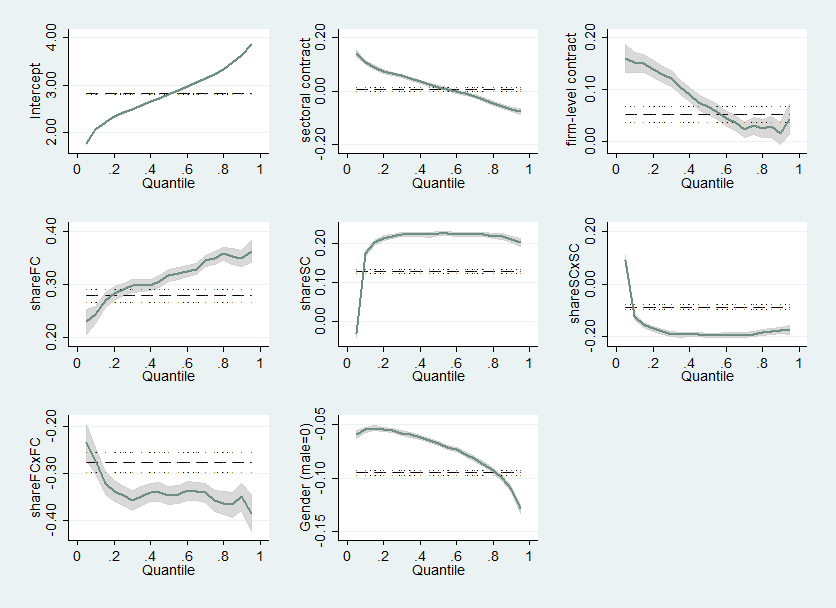
\includegraphics[width=195mm,scale=0.5]{finaldraft}\\
    \label{Fig:CQROLS}
    \footnotesize Data source: GSES 2010
  \end{center}
\end{figure}
\end{landscape}



\subsection{Unconditional Quantile Regression}\label{SubSec:UQR}


\subsubsection{Theory}
Since the conditional quantile regression approach is used to estimate the impact of a covariate on a quantile of the outcome variable, conditional on the distribution of other covariates, it lacks generalizability and the interpretation of the estimated treatment effects across quantiles becomes problematic.
Conversely, the unconditional quantile regression approach, firstly introduced by \cite{Firpo&Fortin&Lemieux:09}, marginalizes the effect over the distributions of other covariates and hence, overcomes the limitations of the conditional quantile regression approach. It is therefore advisable to use the unconditional quantile regression approach if the model contains multiple covariates and interaction effects. Unconditional quantile regressions are applicable to many research fields and have for example been used to investigate the determinants of medication adherence \citep{Borah&Basu:2013} or the effect of cigarette tax increases on smoking behavior \citep{Maclean&Marti&Webber:2014}.

There are several ways to generalize the effect of a covariate on the unconditional quantile of the outcome variable. One option is to use the coefficient estimates of the conditional quantile regression in order to recover equation \ref{4}. \cite{Firpo&Fortin&Lemieux:09} show that the unconditional quantile partial effect of a covariate $X$ on $Y$, $UQPE(\tau)$, equals a weighted average (over the distribution of $X$) of the partial effect of $X$, $CQPE(\zeta_{\tau}, X)$, on a specific conditional quantile $\zeta_{\tau}(X)$ of $Y$, corresponding to the $\tau$-th unconditional quantile of the distribution of $Y$, that we are interested in. In general, it holds true that the conditional quantile partial effect of $X$ does not average up to the effect on the same unconditional quantile, $UQPE(\tau) \neq \E[CQPE(\tau, X)]$.\footnote{ except for a linear, additively separable model} In order to gain a better understanding of the relationship between conditional and unconditional quantile partial effects let us assume that we are interested in the $UQPE$ for the median of the wage distribution, $UQPE(\tau = 0.5)$. If union coverage had a positive effect on wages, the overall median would perhaps correspond to the $25^{th}$ percentile of those covered by a union, and to the $75^{th}$ percentile of those not covered by a union: $\zeta_{0.5}(X=1)=0.25$ and $\zeta_{0.5}(X=0)=0.75$. The average of the two conditional quantile partial effects results in the unconditional quantile partial effect at the median, whereas taking the average of the medians of the two conditional quantiles may yield a different result. Hence, this approach can only be implemented if the unconditional quantiles of $Y$ can be mapped to the corresponding conditional quantiles under different conditioning arguments, which is often not feasible \citep{Borah&Basu:2013}.

The recently introduced approach by \cite{Firpo&Fortin&Lemieux:09} uses the concept of recentered influence functions (RIFs) to perform unconditional quantile regressions. The influence function is a statistical tool applicable to robust estimation of econometric models and defined as
\begin{equation}\label{8}
  IF(y;v(F))=\lim_{\epsilon \rightarrow 0}\frac{[v((1-\epsilon)F+\epsilon \delta_{y})-v(F)]}{\epsilon} , 0 \leq \epsilon \leq 1
\end{equation}
where $F$ is the sample probability distribution of $Y$ and $\delta_y$ represents the distribution for a point mass at the value $y$. Hence, the mixture distribution $(1-\epsilon)F + \epsilon \delta_{y}$ consists of the actual distribution $F$ weighted by $(1-\epsilon)$ and the value $y$ weighted by $\epsilon$. The influence function therefore assesses the marginal influence of an observation at the value $y$ on the distributional statistic $v(F)$. The recentered influence function is obtained by adding back the distributional statistic $v(F)$ to its influence function:
\begin{equation}\label{9}
  RIF(y;v)=v(F)+IF((y;v)
\end{equation}
One advantageous property of the recentered influence function is that its expectation equals the distributional statistic $v(F)$: $\E[RIF(y;v)]=v(F)$. Take for example the mean, $\mu$ as the statistic of interest, then, using L'H\^opital's rule: \footnote{ $\lim_{\epsilon \rightarrow 0}\frac{[(1-\epsilon)\mu + \epsilon y -\mu]}{\epsilon} = \frac{''0''}{''0''} \longrightarrow$ L'H\^opital's rule yields: $\frac{f'(\epsilon)}{g'(\epsilon)}=\frac{-\mu + y}{1}=y-\mu$}
\begin{equation}\label{10}
  RIF(y;\mu)=\mu + \lim_{\epsilon \rightarrow 0}\frac{[(1-\epsilon)\mu + \epsilon y -\mu]}{\epsilon}=\mu +(y-\mu)=y
\end{equation}
\begin{equation*}\label{11}
  \E[RIF(y;\mu)]=\mu
\end{equation*}
Then, the recentered influence function yields the value of Y itself, implying that regressing the recentered influence function for the mean on $X$ yields the same coefficients as an ordinary least squares regression.\\
Now, let us change the statistic of interest to a specific quantile $\tau$ of the outcome distribution and determine the influence function. Therefore, we denote the quantile of the mixture distribution as:
\begin{equation}\label{12}
  q_{\tau}((1-\epsilon)F+\epsilon \delta_{y})=q_{\tau}^{'}
\end{equation}
We have
\begin{equation*}
  (1-\epsilon)F(q_{\tau}^{'})+\epsilon \delta_{y}(q_{\tau}^{'})=\tau
\end{equation*}
with $\delta_{y}(q_{\tau}^{'})=I(Y\leq q_{\tau}^{'})$, a dummy variable determining whether the outcome variable is below $q_{\tau}$. Using the implicit function theorem leads us to:
\begin{equation*}\label{13}
  \frac{\partial q_{\tau}^{'}}{\partial \epsilon}=-\frac{-F(q_{\tau}^{'})+I(Y \leq q_{\tau}^{'})}{(1-\epsilon)f_{Y}(q_{\tau}^{'})}
\end{equation*}
For $\epsilon \rightarrow 0$, $q_{\tau}^{'} \rightarrow q_{\tau}$ and $F(q_{\tau}^{'}) \rightarrow \tau$
\begin{equation}\label{14}
  IF(y;q_{\tau})=\frac{\tau - I(Y \leq q_{\tau})}{f_{Y}(q_{\tau})}
\end{equation}
where $q_{\tau}$ represents the $\tau$-th quantile of the unconditional distribution of $Y$ and $f_{Y}(q_{\tau})$ refers to the probability density function of $Y$. Consequently, the recentered influence function is:
\begin{equation}\label{15}
  RIF(y;q_{\tau})=q_{\tau}+IF(y;q_{\tau})=q_{\tau} + \frac{\tau - I(Y \leq q_{\tau})}{f_{Y}(q_{\tau})}
\end{equation}
\cite{Firpo&Fortin&Lemieux:09} call the expectation of the $RIF(Y; v,F_{Y})$, conditional on the explanatory variables $X$, the \emph{RIF regression model}, $\E[RIF(Y; v, F_{Y})|X]=m_{v}(X)$. Constructed for quantiles, $\E[RIF(Y; q_{\tau,} F_{Y})|X]=m_{\tau}(X)$ represents an \emph{unconditional quantile regression}. Furthermore, they show that the average derivative of the unconditional quantile regression, $\E[m_{\tau}^{'}(X)]$, can be interpreted as the marginal effect on the unconditional quantile of interest, resulting from a small location shift in the distribution of covariates, ceteris paribus. Similarly to an OLS regression, the recentered influence function can be regressed on the set of covariates $X$. Therefore, we need to estimate
\begin{equation*}
  \widehat{RIF}(Y; \hat{q}_{\tau})=\hat{q}_{\tau}+ \frac{\tau - I(Y \leq \hat{q}_{\tau})}{\hat{f}_{Y}(\hat{q}_{\tau})}.
\end{equation*}
The estimated density of $Y$, $\hat{f}_{Y}(\hat{q}_{\tau})$ can be obtained by using, for example, the kernel density estimator, whereas $\hat{q}_{\tau}$ is determined by estimating the unconditional quantile $\tau$, based on the sample at hand.

After presenting the microeconomic foundations of collective bargaining as well as introducing the methods of my econometric investigation, I will describe the used dataset and present the regression results in the following sections.

\subsubsection{Implementation}

\subsubsection{Testing - Unconditional Quantile Regression Results}

The results of the unconditional quantile regression are displayed in table \ref{UQR} and the resulting unconditional average partial effects are summarized in table \ref{APEs:UQR}. Similarly to the OLS regression, the coefficients of the quantile regression can now be interpreted as effects on the unconditional wage distribution.

Compared to the conditional quantile regression estimates, the coefficients obtained by an unconditional quantile regression have significantly larger spreads across the wage distribution. For example, the individual union wage premium for an employee, covered by a sectoral contract in a firm with an average coverage ratio, declined monotonically from $6.4\%$ at the 10th percentile to $-0.131\%$ at the 90th percentile in a conditional quantile regression setting. In contrast, the average partial effect for individual coverage at the sectoral level decreases from $19.2\%$ at the 10th percentile to $-43\%$ at the 90th percentile of the unconditional wage distribution. This means that an employee, working under a sectoral collective contract in a firm with an average coverage ratio earns on average $19.2\%$ more than an uncovered employee in the same firm, at the 10th percentile. At the top end of the wage distribution (90th percentile), the uncovered employee earns on average $43\%$ more than the covered employee. The reason for that trend may be that firms want to pay a premium to highly productive employees, e.g. employees with management responsibilities. Furthermore, these employees cannot rely on a collective contract as a fall back position and are therefore paid a risk premium, as argued in earlier sections. Similar results are obtained for firm-level coverage, although the effects are estimated to be less drastic, meaning that the union wage premium for covered employees at the bottom end of the distribution is less than under a sectoral contract. In return, the negative union wage premium at the top of the distribution is lower than under sectoral bargaining coverage as well ($-19.4\%$ under firm-level coverage, compared to the $43\%$ under sectoral level coverage, at the 90th percentile).
\begin{landscape}
\begin{table}[]
\scriptsize
\centering
\caption{Unconditional Quantile Regression Results}
\label{UQR}
\begin{tabular}{l|cccccccccc}
 percentile & \multicolumn{2}{c}{(10)} & \multicolumn{2}{c}{(25)} & \multicolumn{2}{c}{(50)} & \multicolumn{2}{c}{(75)} & \multicolumn{2}{c}{(90)}\\
\hline
 & coef. & std. err. & coef. & std. err. & coef. & std. err. & coef. & std. err. & coef. & std. err. \\
\hline
Sector Contract (SC)    & $0.176^{**}$ & $(0.007)$ & $0.012^{*}$ & $(0.005)$ & $0.029^{**}$ & $(0.004)$ & $-0.020^{**}$ & $(0.005)$ & $-0.139^{**}$ & $(0.006)$\\
Firm Contract (FC)      & $0.184^{**}$ & $(0.013)$ & $0.111^{**}$ & $(0.010)$ & $0.069^{**}$ & $(0.011)$ & $0.108^{**}$ & $(0.015)$ & $-0.151^{**}$ & $(0.185)$\\
shareSC                 & $-0.004$ & $(0.006)$ & $0.058^{**}$ & $(0.003)$ & $0.050^{**}$ & $(0.003)$ & $0.304^{**}$ & $(0.005)$ & $0.806^{**}$ & $(0.010)$\\
shareFC                 & $0.124^{**}$ & $(0.012)$ & $0.118^{**}$ & $(0.007)$ & $0.100^{**}$ & $(0.006)$ & $0.356^{**}$ & $(0.010)$ & $0.857^{**}$ & $(0.022)$\\
shareSCxSC              & $0.045^{**}$ & $(0.010)$ & $0.103^{**}$ & $(0.006)$ & $-0.020^{**}$ & $(0.005)$ & $-0.331^{**}$ & $(0.008)$ & $-0.816^{**}$ & $(0.012)$\\
shareFCxFC              & $-0.064^{**}$ & $(0.019)$ & $-0.052^{**}$ & $(0.014)$ & $-0.114^{**}$ & $(0.014)$ & $-0.521^{**}$ & $(0.020)$ & $-0.803^{**}$ & $(0.031)$\\
gender (male=0)         & $-0.048^{**}$ & $(0.002)$ & $-0.038^{**}$ & $(0.002)$ & $-0.057^{**}$ & $(0.001)$ & $-0.121^{**}$ & $(0.002)$  & $-0.164^{**}$ & $(0.002)$\\
\hline
$N$                     & \multicolumn{2}{c}{552750} & \multicolumn{2}{c}{552750} & \multicolumn{2}{c}{552750} & \multicolumn{2}{c}{552750} & \multicolumn{2}{c}{552750} \\
\hline
\end{tabular}\\
\bigskip
Unconditional quantile regression includes a full set of firm-specific and individual-worker covariates.\\
$^{*}$/$^{**}$: significance at the 5\%/1\% -level
\end{table}
\end{landscape}
The average partial effects for an increase in the share of covered employees within a firm, under both coverage regimes, are different from the effects obtained in table \ref{APEs:CQR}. While there is no real trend noticeable at lower quantiles, the effects become larger at the top end of the wage distribution for both coverage regimes. For example, a $10\%$ increase in the share of covered employees by a sectoral contract in a firm with an average coverage rate, leads to a $0.12\%$ increase in wages at the 10th percentile and a $5.15\%$ increase at the 90th percentile of the unconditional wage distribution, compared to effects of $1.3\%$ at the 10th percentile and $1.49\%$ at the 90th percentile of the conditional wage distribution. Therefore, an increasing share of covered employees contributes to wage dispersion.

Whereas the interaction coefficients are negative at all quantiles and only tendentially declining across quantiles in table \ref{CQR}, they decrease significantly more using unconditional quantile regression, and are even positive for sectoral coverage on lower quantiles. Hence, the effect of individual coverage by a sectoral contract in high coverage firms is particularly positive for employees on lower quantiles (e.g. $22.1\%$ at the 10th percentile)\footnote{ $\beta_{SC}^{(10)}+\beta_{shareSCxSC}^{(10)} \cdot 100\%=0.176+0.045=22.1\%$} and particularly negative for employees on higher quantiles (e.g. $-95.5\%$ at the 90th percentile).\footnote{ $\beta_{SC}^{(90)}+\beta_{shareSCxSC}^{(90)} \cdot 100\%=-0.139-0.816=-95.5\%$} For individual coverage by a firm-specific contract in a high-coverage firm, union wage premiums are negatively affected on all quantiles, i.e. the interaction effect reduces the union wage premium in high coverage firms, compared to low coverage firms. This reduction is particularly high on the upper end of the unconditional wage distribution.

Similarly to the conditional quantile regression results, the unconditional quantile regression results yield a significant gender wage gap on all quantiles. However, the gender wage gap remains fairly constant up until median-wages. Towards the upper end of the wage distribution, the gender wage gap turns out much larger than predicted by conditional quantile regression. Women earn $16.4\%$ less than men on the 90th percentile of the wage distribution, compared to $11.1\%$ at the 90th percentile of the conditional wage distribution.

\begin{table}[]
\scriptsize
\centering
\caption{Average Partial Effects obtained by Unconditional Quantile Regression}\vspace{0.2cm}
\label{APEs:UQR}
\begin{tabular}{l|ccccc}

                    & $(10)$ & $(25)$ & $(50)$ & $(75)$ & $(90)$ \\
  \hline
  Sector Contracts  & $0.192$ & $0.049$ & $0.022$ & $-0.138$ & $-0.430$ \\
  Firm Contracts    & $0.181$ & $0.108$ & $0.063$ & $0.080$ & $-0.194$ \\
  shareSC           & $0.012$ & $0.095$ & $0.043$ & $0.186$ & $0.515$ \\
  shareFC           & $0.121$ & $0.115$ & $0.094$ & $0.328$ & $0.814$ \\
  \hline
\end{tabular}
\end{table}

\subsection{Conclusion}
